%%%%%%%%%%%%%%%%%%%%%%%%%%%%%%%%%%%%%%%%%%%%%%%%%%
\section{Event Reconstruction}
%%%%%%%%%%%%%%%%%%%%%%%%%%%%%%%%%%%%%%%%%%%%%%%%%%
\subsection{Noise Reduction}

Figure \ref{Fig:beforeFFT} shows raw waveform of the TPC signal
before applying any noise reduction. Two waveforms shown in this plot
are channel 13 and 37 in Figure~\ref{Fig:Textbook} which are roughly
proton stopped point and electron shower maximum point, respectively.
Signal-to-noise ratio for this particular case is poor and pion signal 
which is supposed to be t=400 $\mu$s is almost hidden by the noise. 
While time width of TPC signal is few $\mu$s which is determined by
drift time between anode and anode-grid, dominant noise component looks
higher frequency. To reduce such noises, we have applied FFT 
(Fast Flourier Transformation) filter to cut the high frequency component.
Figure \ref{Fig:FFT} shows amplitude as a function of frequency
for the same event. This clearly shows dominant noise component with
$>$ 200 kHz has good separation with signal component ($<$ 100 kHz).
Figure \ref{Fig:afterFFT} shows the waveform after removing high frequency
($>$ 80 kHz) component by the FFT filter. Signal-to-noise ratio is dramatically
improved. On the other hand, we expect certain bias to the signal charge
measurement by this filter, and it will be discussed in Section x.

\begin{figure}[htbp]
 \begin{center}
  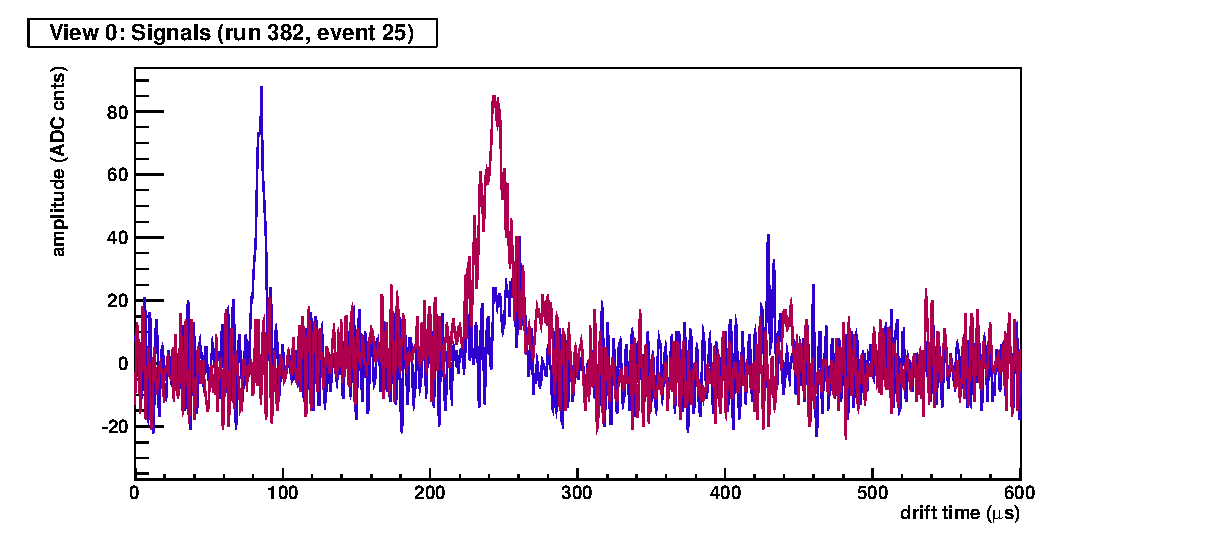
\includegraphics[width=100mm]{fig/beforeFFT.eps}
 \end{center}
 \caption{TPC raw signal waveform for "Textbook" event channel 13 and 37.}
 \label{Fig:beforeFFT}
\end{figure}

\begin{figure}[htbp]
 \begin{center}
  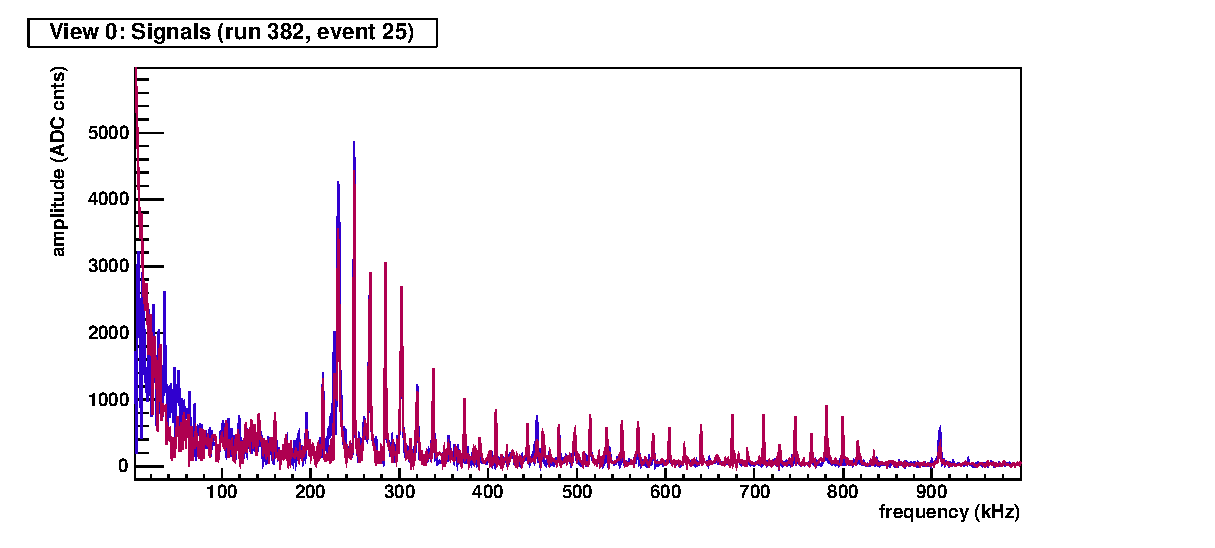
\includegraphics[width=100mm]{fig/FFT.eps}
 \end{center}
 \caption{FFT frequency amplitude distribution}
 \label{Fig:beforeFFT}
\end{figure}

\begin{figure}[htbp]
 \begin{center}
  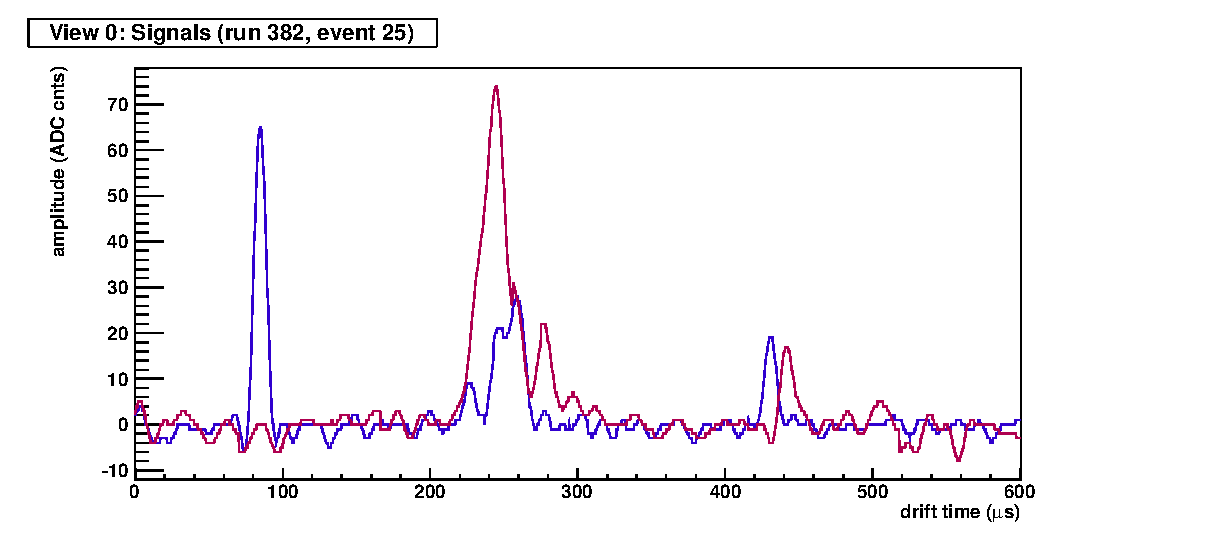
\includegraphics[width=100mm]{fig/afterFFT.eps}
 \end{center}
 \caption{TPC signal waveform after cutting the frequency $>$ 80 kHz.}
 \label{Fig:afterFFT}
\end{figure}


%\subsection{Hit Finding/Clustering}
\subsection{Hit Finding/Clustering}
After noise reduction we find signal hits and create clusters associated to single tracks. 
Hit is defined as bump over given threshold in a channel. 
After finding all hits in an event, we construct cluster by merging adjacent hits. 
The example of hit finding and clustering is shown in Fig~\ref{fig:Clustering}, which indicates reasonable hit and cluster findings. 
Threshold of hit finding is 6 ADC counts, which is about 2.5$\sigma$ from typical data noise level (as shown in Fig~\ref{Fig:beforeFFT}) and keeping more than 99\% of Kaon hit finding efficiency from simulation.
% noise level from outside window of PhysicsOct55 (rms~2.49)
ADC count distribution is fitted by step funcion plus Gaussian to estimate the charge of hit in ADC $\times$ $\mu$s unit.
Fitting $\chi^2 < 3$ and $2.5<$~(time~width~of~hit)~$<8$~$\mu$s are required to remove noise hits further.

\begin{figure}[htbp]
 \begin{center}
  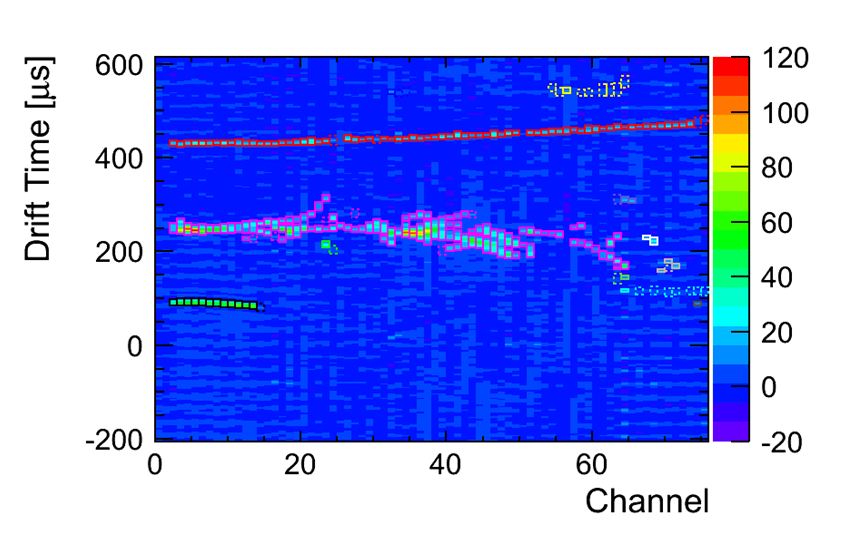
\includegraphics[width=100mm]{fig/clustering.eps}
 \end{center}
 \caption{Example of hit finding and clustering. A colored box corresponds to a hit and colors represent different clusters.}
 \label{fig:Clustering}
\end{figure}

%\begin{itemize}
%\item Plot: Finding efficiency vs threshold (Naganoma): TBU
%\item Plot: Through-going pion data Q vs pion (Tanaka)
%\end{itemize}


\begin{figure}[htbp]
 \begin{center}
  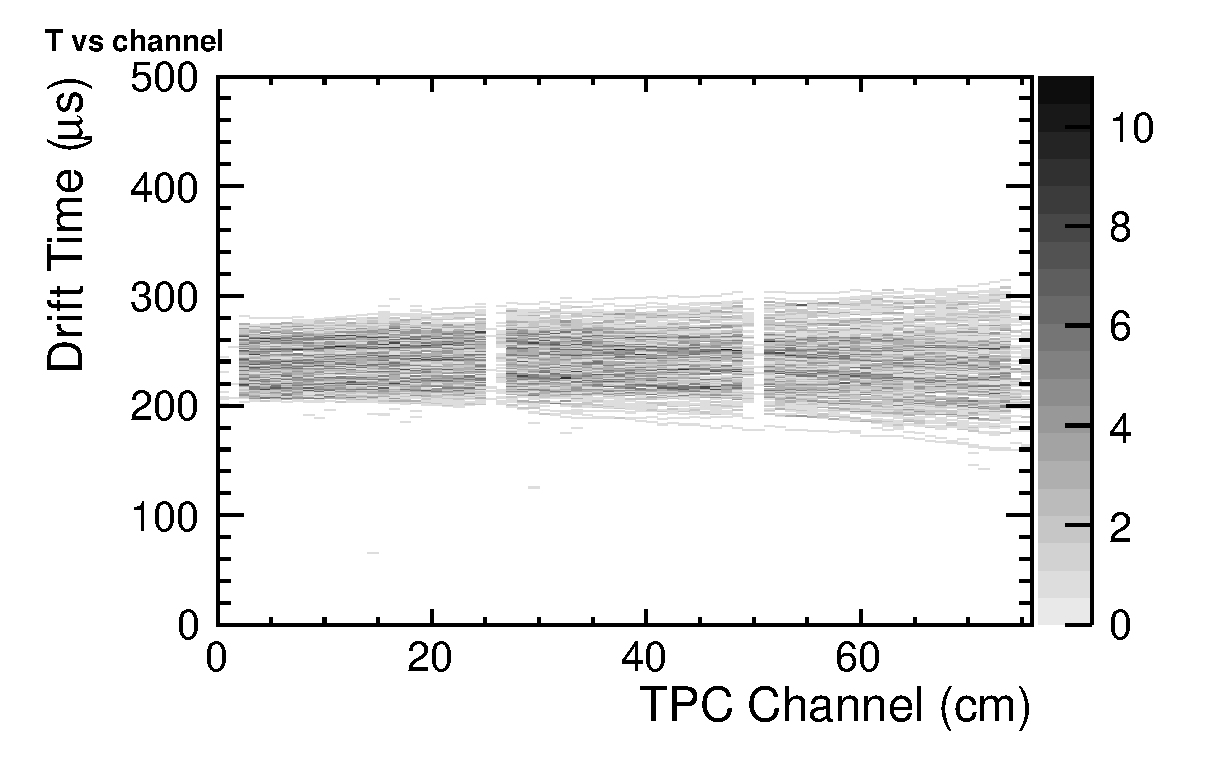
\includegraphics[width=100mm]{fig/PionTrack.eps}
 \end{center}
 \caption{800 MeV/c pion sample}
 \label{fig:PionTrack}
\end{figure}

\begin{figure}[htbp]
 \begin{center}
  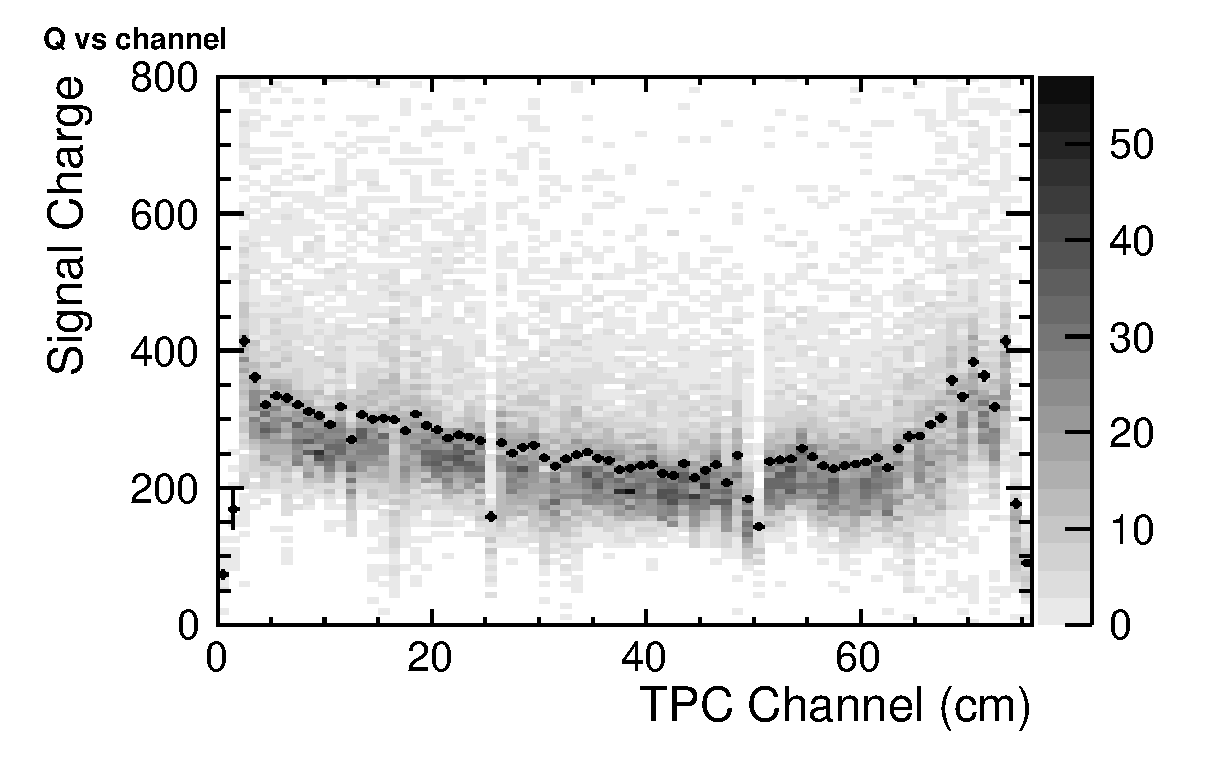
\includegraphics[width=100mm]{fig/PionQvsCh.eps}
 \end{center}
 \caption{800 MeV/c pion average hit charge}
 \label{fig:PionQvsCh}
\end{figure}

\begin{figure}[htbp]
 \begin{center}
  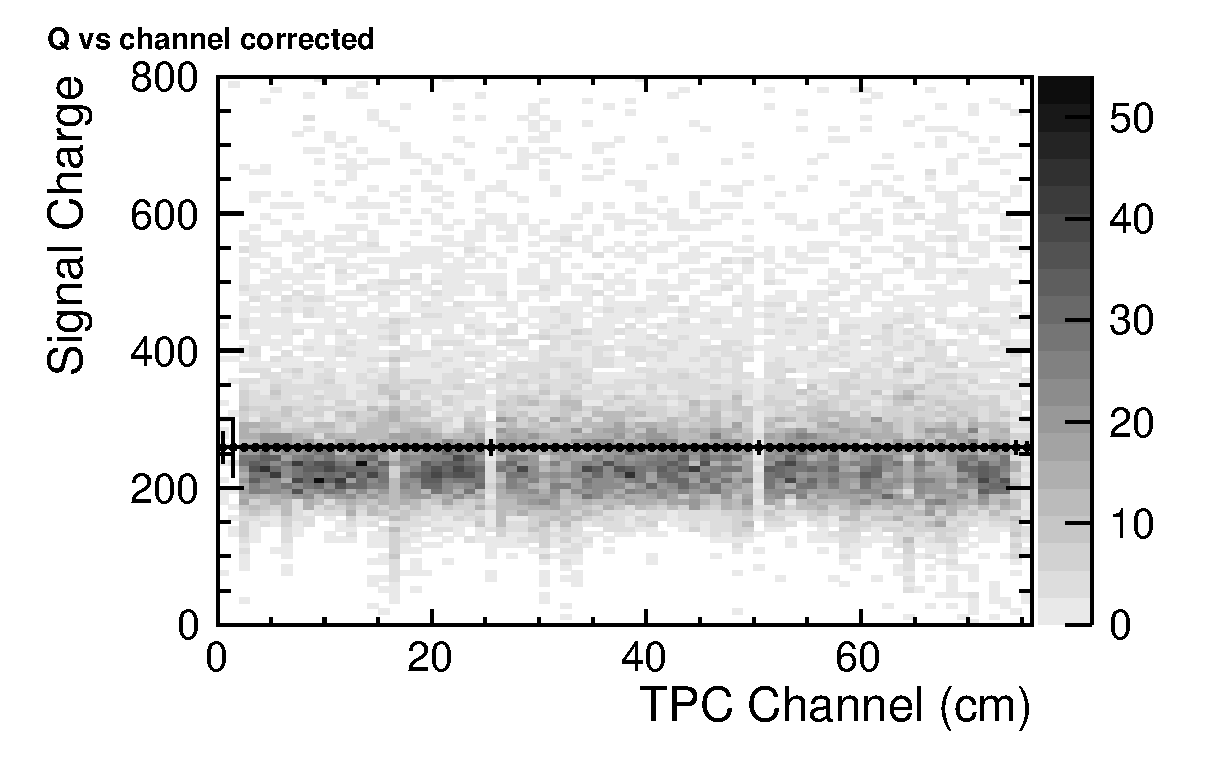
\includegraphics[width=100mm]{fig/PionQcvsCh.eps}
 \end{center}
 \caption{800 MeV/c pion average hit charge after calibration}
 \label{fig:PionQcvsCh}
\end{figure}

\subsection{Stopped Point Finding}
%\subsubsection{Proton}
%\subsubsection{Proton}

Figure\ref{fig:Proton_Event_Display} shows typical EventDisplay of Proton.
Proton has simple structure of events, that is,
as Proton doesn't decay any particles, so it is easy to define stopped point.\\
First, We define `max channel` and `max charge channel` event by event
(then,required single cluster for single event).
`Max channnel` is the channel number of hit which has the most large channel number in the cluster,
and `max charge channel' is the channel number of hit which has the most large amount of signal.
We select events in either following two situations, and define `max channel` as stopped point.

\begin{itemize}
\item max channel $=$ max charge channel \\
\item max channel $=$ max charge channel $+$ 1\\
\end{itemize}

\begin{figure}[htbp]
  \centering
  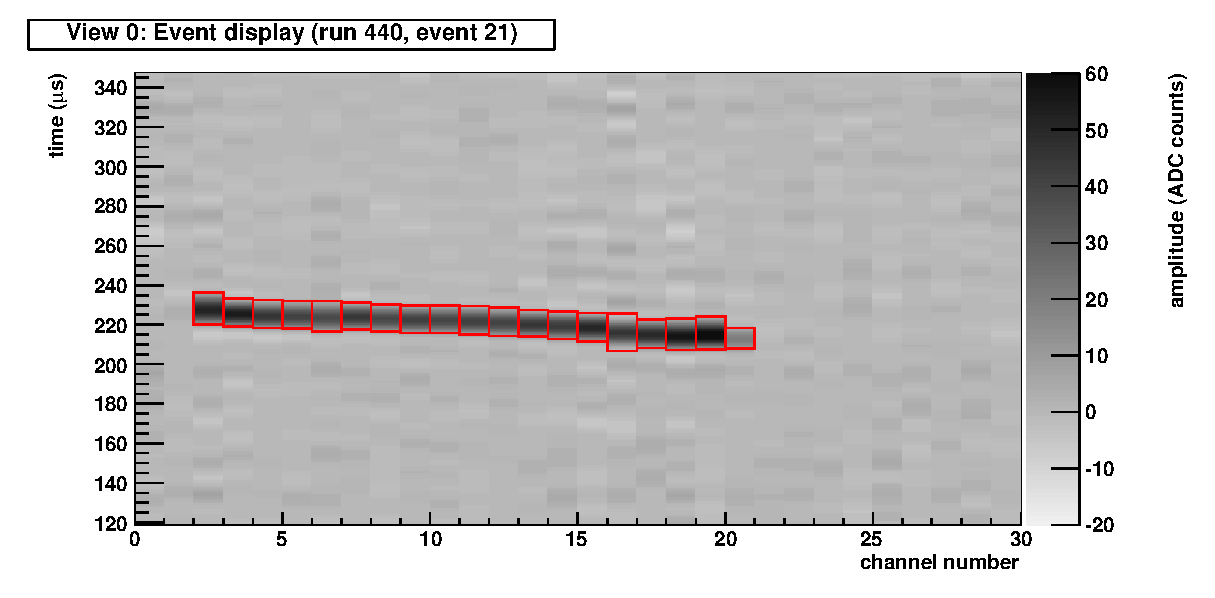
\includegraphics[width=10cm,clip]{./fig/Display_run440_ev21.eps}
  \caption{Typical Event Display of Proton}
  \label{fig:Proton_Event_Display}
\end{figure}

%\subsection{Stopped Kaon}
\subsection{Stopped Kaon}
Hough transform was invented for machine analysis of bubble chamber photographs by Paul.V.C.Hough.\cite{3069654}
We find straight lines using hough method , and find Kaon stopped point from the intersection of straight lines.\\
Figure \ref{hmap2} shows hit map like a Kaon track.
One point in the X-Y space can be transformed into sinusoidal curve in the $\rho$-$\theta$ space.Figure \ref{rho_theta2} shows sinusoidal curves in all points.
And, we find the straight line associated with the largest number of points by choosing the most dense point in $\rho$-$\theta$ space.
Next , the sinusoidal curves of the hits associated with frist straight line are removed from figure \ref{rho_theta2}.
Figure \ref{rho_theta3} shows sinusoidal curves after the hits associated with frist straight line removed.
We find second straight line using the same procedure.This procedure is repeated until there are less than three points.Figure \ref{hmap_fit} shows the two straight lines found by hough transform mehotd.\\
Kaon stopped point in the liquid argon detecor defined as charge maximum point around the intersection of some lines.


\begin{figure}[!htb]
  \begin{minipage}{0.5\hsize}
    \begin{center}
      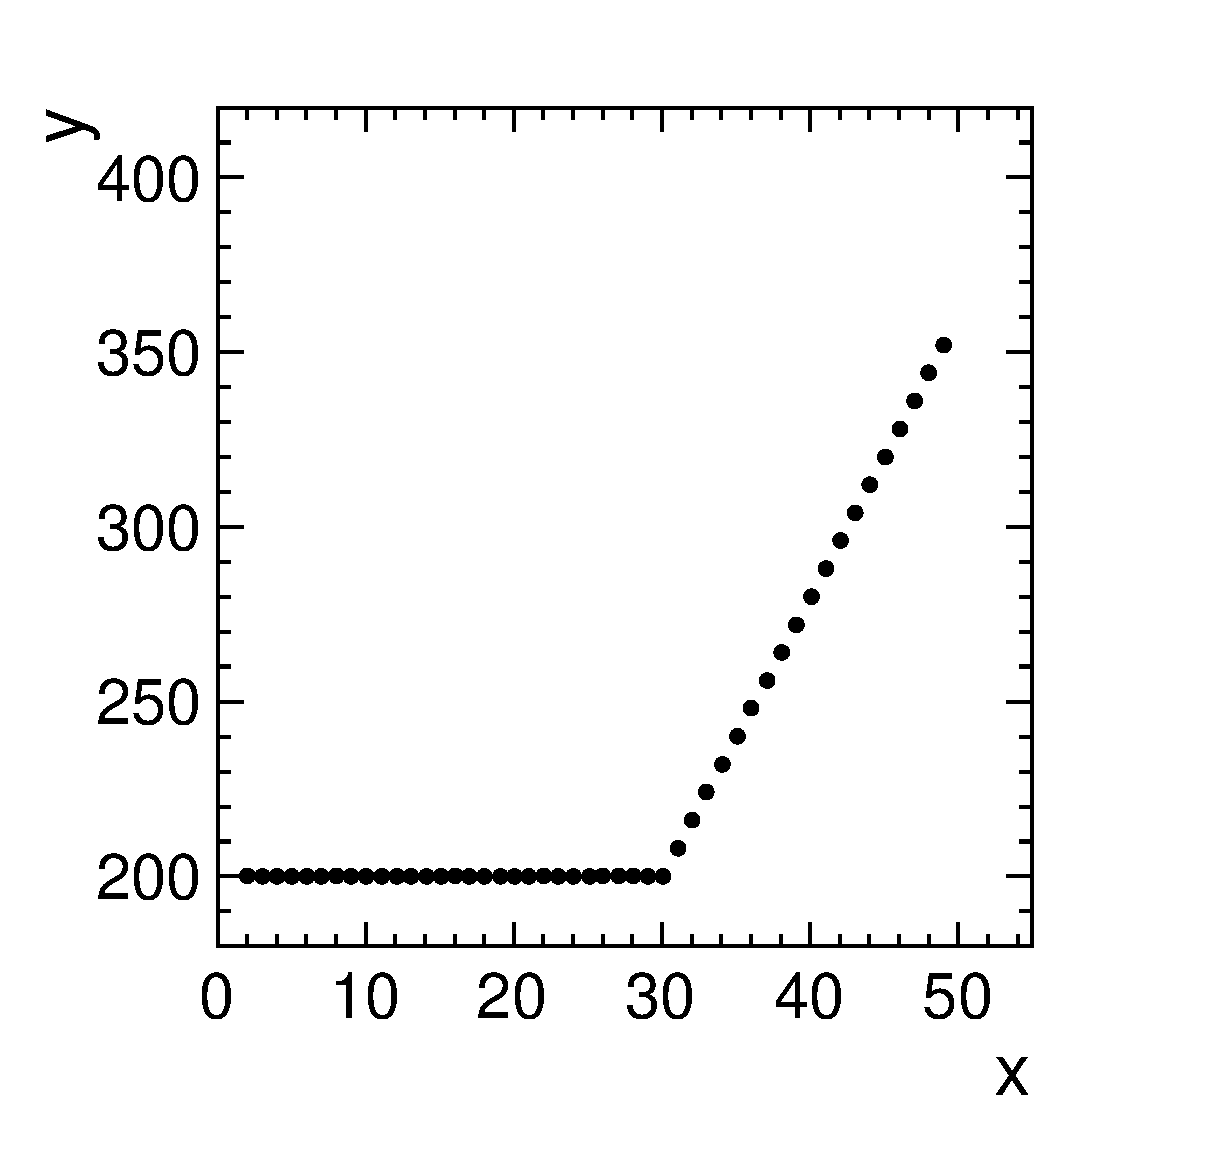
\includegraphics[width=35mm]{fig/hmap2.eps}
    \end{center}
    \caption{Hit map like a Kaon track}
    \label{hmap2}
  \end{minipage}
  \begin{minipage}{0.5\hsize}
    \begin{center}
      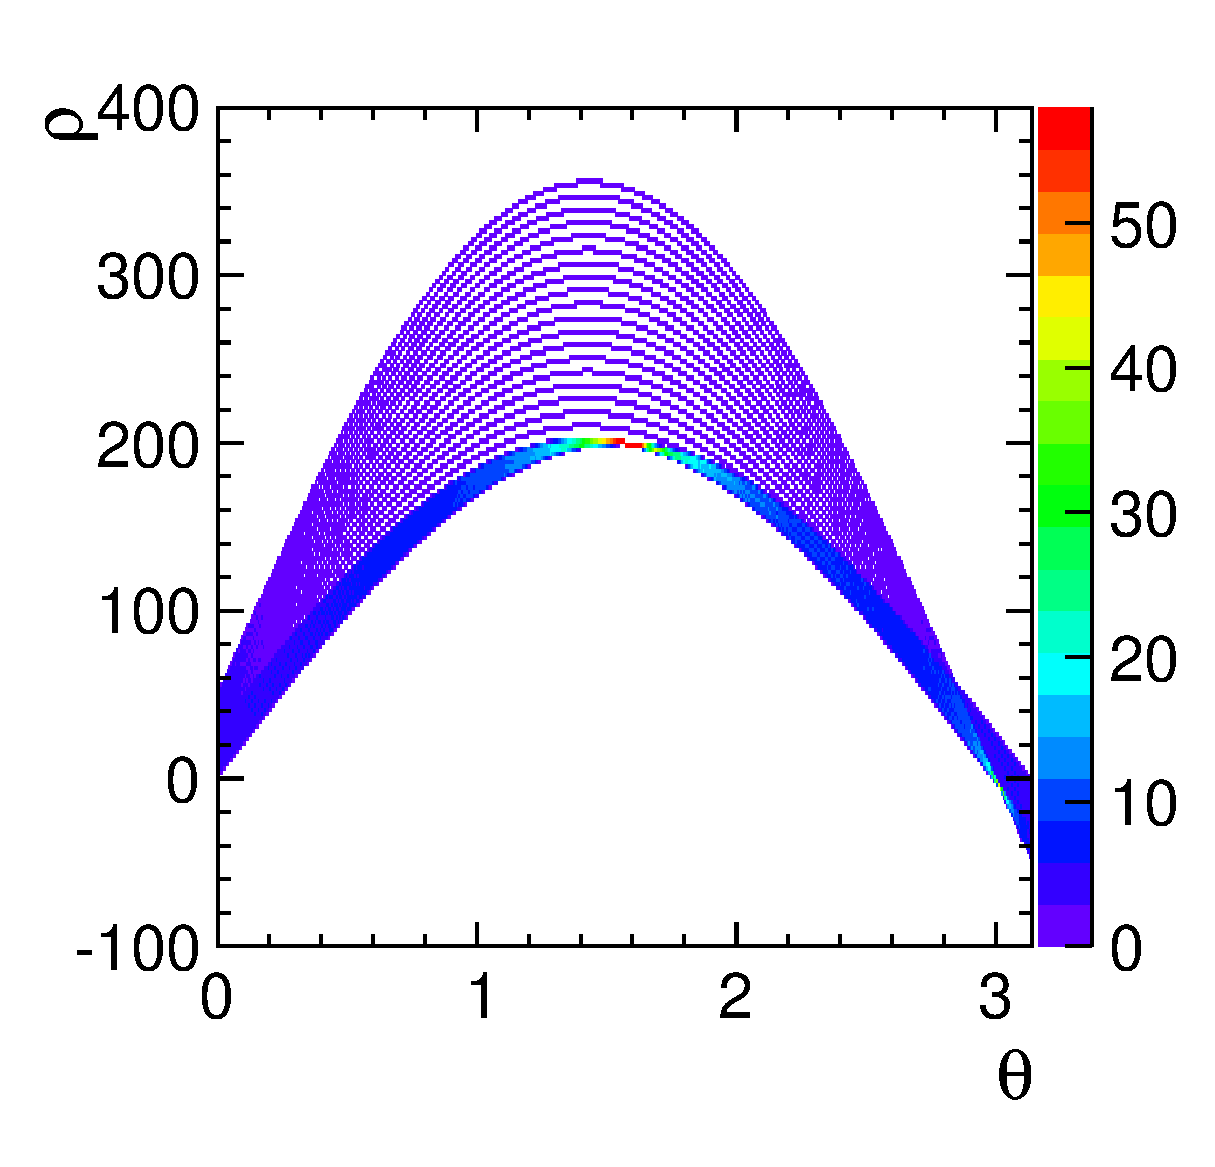
\includegraphics[width=35mm]{fig/rho_theta2.eps}
    \end{center}
    \caption{sinusoidal curves getting form all hough transformed  points of Figure \ref{hmap2}}
    \label{rho_theta2}
  \end{minipage}
  \\
  \begin{minipage}{0.5\hsize}
    \begin{center}
      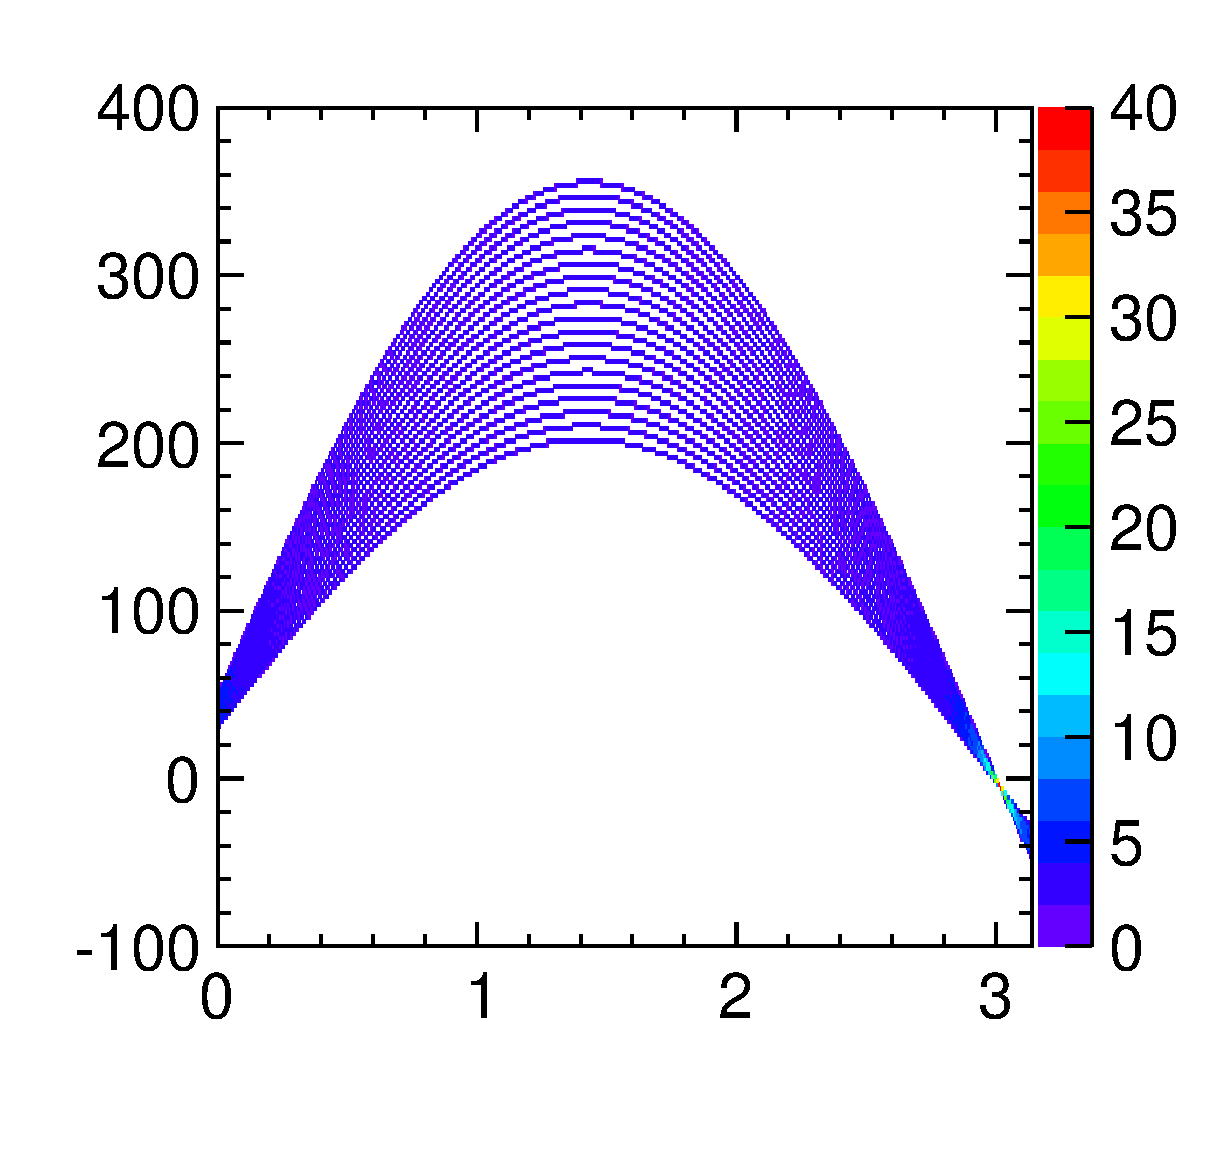
\includegraphics[width=35mm]{fig/rho_theta_kink.eps}
    \end{center}
    \caption{sinusoidal curves removed the points associated with first straight line from figure \ref{rho_theta2}}
    \label{rho_theta3}
  \end{minipage}
  \begin{minipage}{0.5\hsize}
    \begin{center}
      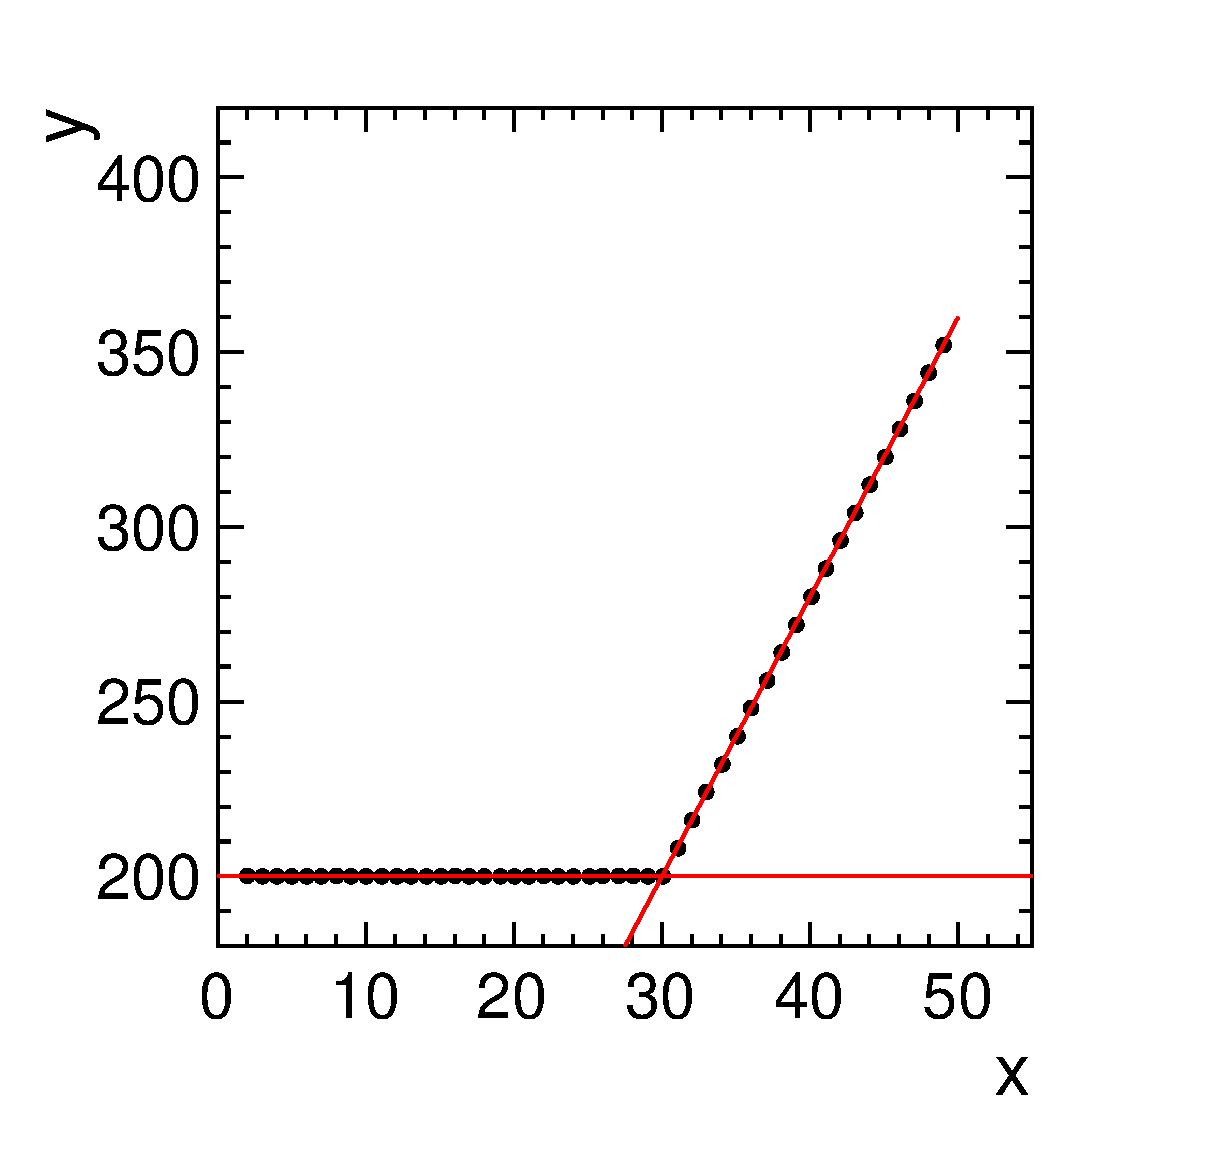
\includegraphics[width=35mm]{fig/hmap_fit.eps}
    \end{center}
    \caption{Two lines found with hough transform method}
    \label{hmap_fit}
  \end{minipage}
\end{figure}


\subsubsection{Chi2 method}
$\chi^{2}$ method is the algorithm that search the point of rapidly increasing fit'$\chi^{2}$ and the point defined as the stopped point.
Because the charged particle coming from upsteam of beam line , track reconstruction is started from minimum channel  to the maximum channel of the cluster.\\
Figure \ref{hmap3} shows hit map like a Kaon track.
We start fitting with straight line from minimum channel to maximum channel.Figure \ref{xvschi} shows range vs fit'$\chi^{2}$ distribution.
As it can be noiced for figure \ref{xvschi}, $\chi^{2}$ is increased rapidly if the straight line is strayed out.
Then , we search the strayed point from the straight line by setting reasonable threhold and draw from minimum channel to the strayed point.
This procedure is done from maximum channel to minimum channel in the same way.
And we draw from maximum channel to the strayed point.
Kaon stopped point in the liquid argon detecor defined as charge maximum point around the intersection of two lines.


\begin{figure}[!htb]
  \begin{minipage}{0.5\hsize}
    \begin{center}
      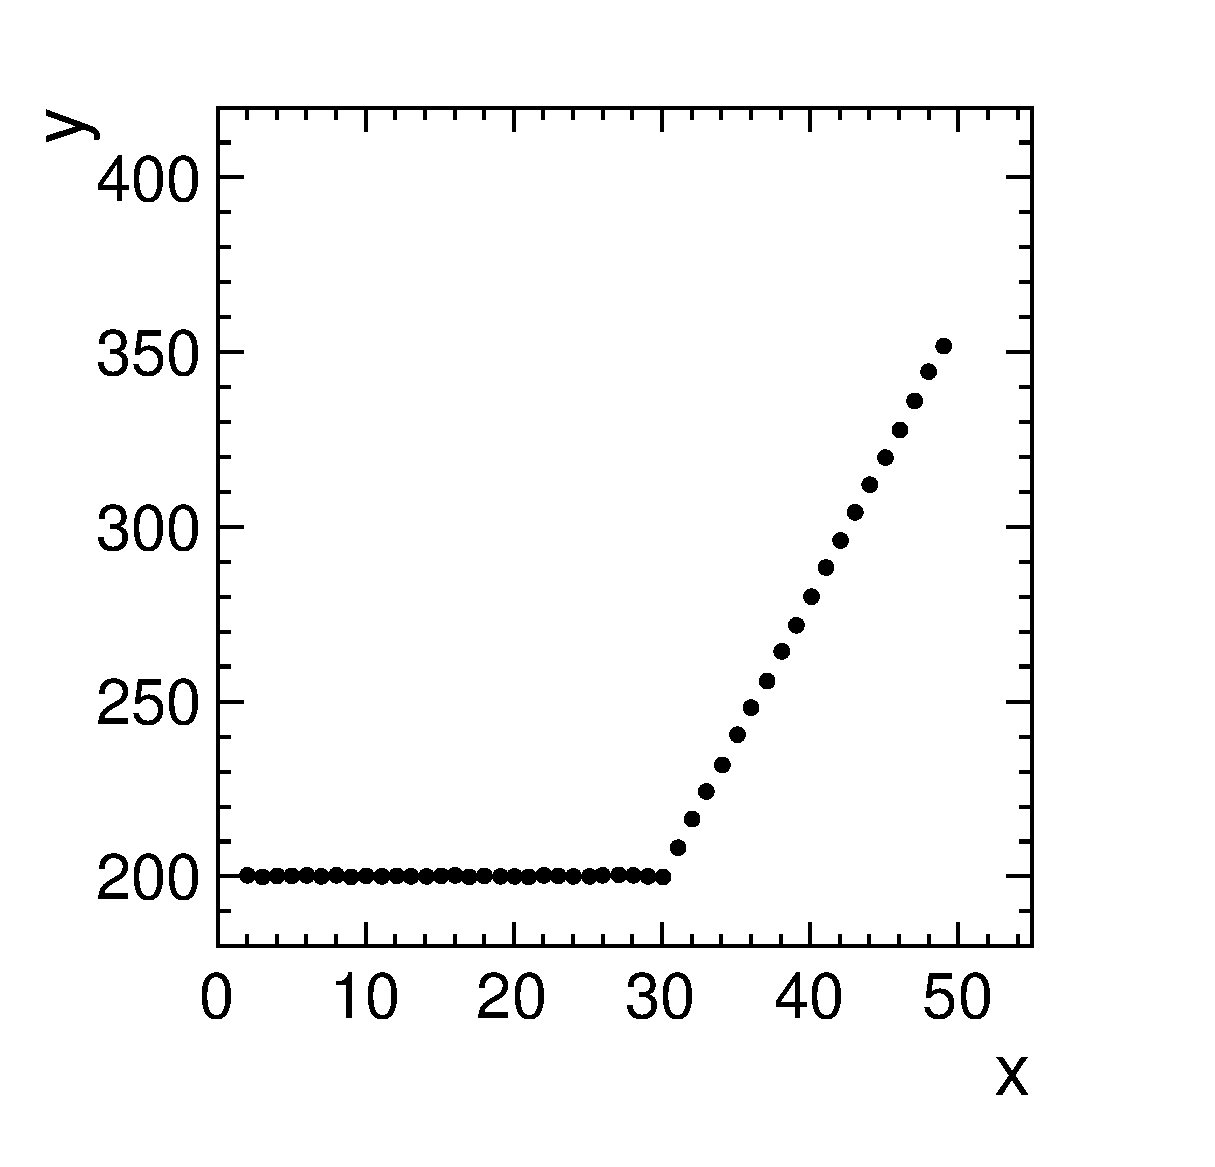
\includegraphics[width=50mm]{fig/hmap_kink_chi2.eps}
    \end{center}
    \caption{hit map like a Kaon track}
    \label{hmap3}
  \end{minipage}
  \begin{minipage}{0.5\hsize}
    \begin{center}
      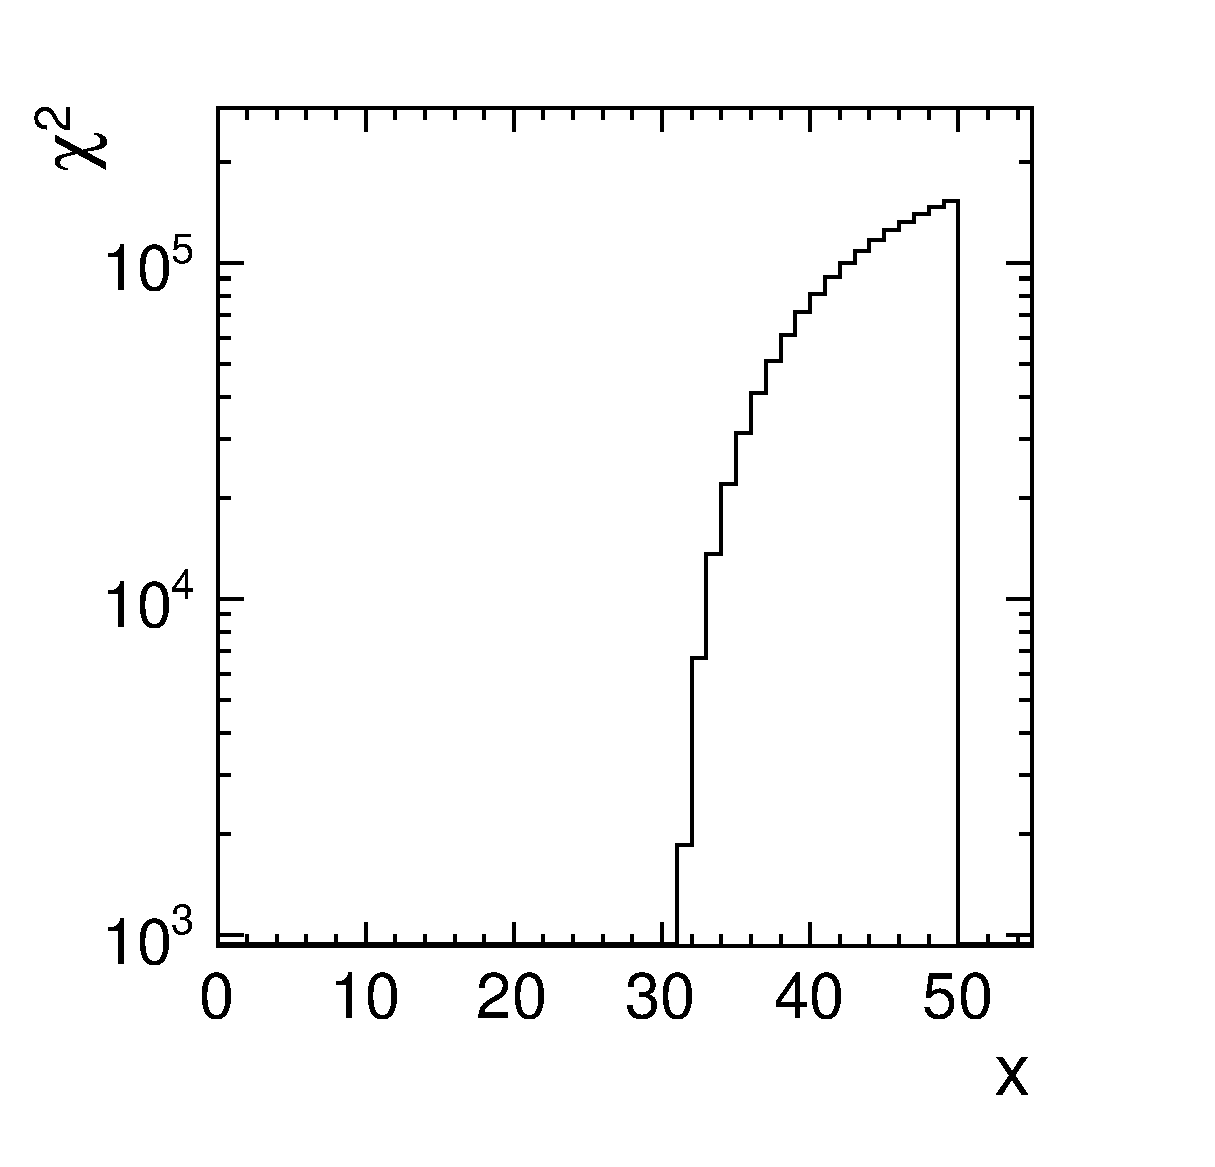
\includegraphics[width=50mm]{fig/chi2_kink_chi2.eps}
    \end{center}
    \caption{range vs $\chi^{2}$ distribution}
    \label{xvschi}
  \end{minipage}
\end{figure}


\subsubsection{BS method}
In the $\chi^{2}$ method , we can't find Kaon stopped point in the case of backward decay.
Then , we find Kaon stopped point using BS method.\\ 
BS method is concept that the Kaon stopped point defined as lightmost channel in the case of backward decay.
we descript below how the track defined as backward decay.
$N_{1}$ is defined as Number of cluster hits found by the clustering.
Stopped point finding is started from minimum channel.
We search for the closet timing hit in next channel from current channel hit. 
Then , we repeat this procedure until maximum channel and count the number of selected hit information($N_{2}$).
In the case of backward decay , $N_{1}$ is larger than $N{2}$.
So , we set reasonable threhold of the difference between $N_{1}$ and $N{2}$ , and if the $N_{1}>N_{2}$ is over the threshold , the track is defined as backward decay.
In the case of backward decay , we defined charge maximum point around the maximum channel as the stopped point. 

\begin{figure}[!htb]
  \begin{center}
    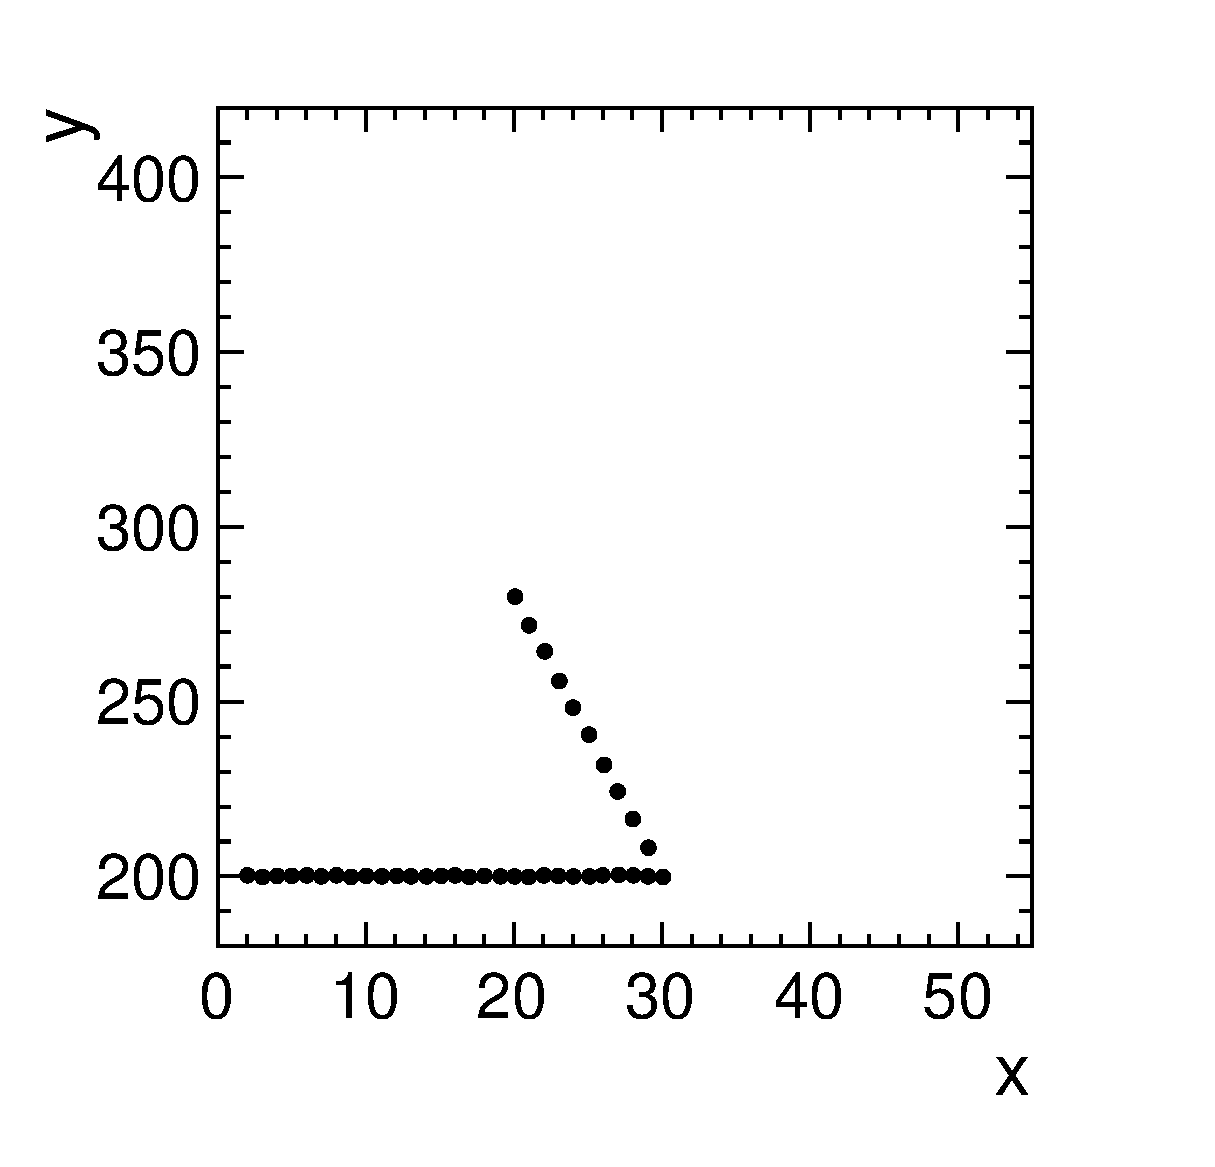
\includegraphics[width=50mm]{fig/hmap_kink_BS.eps}
  \end{center}
  \caption{hit map like a Kaon track}
  \label{hmap_BS}
\end{figure}




